\section{Chandra Kirana Poetra (1174079)}
\subsection{Tugas Membuat Shapefile dengan PySHP}
\begin{enumerate}
	\item No 1
	\lstinputlisting{src/tugas2/1174079/no1.py}
	\begin{figure}[H]
		
\includegraphics[width=6cm]{figures/Tugas2/1174079/no1.PNG}
		\centering
		\caption{Hasil No 1}
	\end{figure}
	\item Nomor 2
	\lstinputlisting{src/tugas2/1174079/no2.py}
	\begin{figure}[H]
		
\includegraphics[width=6cm]{figures/Tugas2/1174079/no2.PNG}
		\centering
		\caption{Hasil No 2}
	\end{figure}
	\item Nomor 3
	\lstinputlisting{src/tugas2/1174079/no3.py}
	\begin{figure}[H]
		
\includegraphics[width=6cm]{figures/Tugas2/1174079/no3.PNG}
		\centering
		\caption{Hasil No 3}
	\end{figure}
	\item Nomor 4
	\lstinputlisting{src/tugas2/1174079/no4.py}
	\begin{figure}[H]
		
\includegraphics[width=6cm]{figures/Tugas2/1174079/no4.PNG}
		\centering
		\caption{Hasil No 4}
	\end{figure}
	\item Nomor 5
	\lstinputlisting{src/tugas2/1174079/no5.py}
	\begin{figure}[H]
		
\includegraphics[width=6cm]{figures/Tugas2/1174079/no5.PNG}
		\centering
		\caption{Hasil No 5}
	\end{figure}
	\item Nomor 6
	\lstinputlisting{src/tugas2/1174079/no6.py}
	\begin{figure}[H]
		
\includegraphics[width=6cm]{figures/Tugas2/1174079/no6.PNG}
		\centering
		\caption{Hasil No 6}
	\end{figure}
	\item Nomor 7
	\lstinputlisting{src/tugas2/1174079/no7.py}
	\begin{figure}[H]
		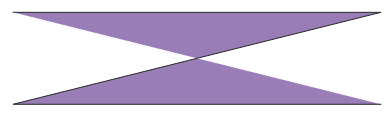
\includegraphics[width=6cm]{figures/Tugas2/1174079/no7.PNG}
		\centering
		\caption{Hasil No 7}
	\end{figure}
	\item Nomor 8
	\lstinputlisting{src/tugas2/1174079/no8.py}
	\begin{figure}[H]
		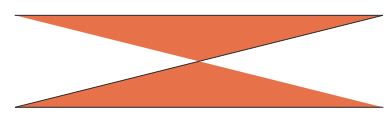
\includegraphics[width=6cm]{figures/Tugas2/1174079/no8.PNG}
		\centering
		\caption{Hasil No 8}
	\end{figure}
	\item Nomor 9
	\lstinputlisting{src/tugas2/1174079/no9.py}
	\begin{figure}[H]
		
\includegraphics[width=6cm]{figures/Tugas2/1174079/no9.PNG}
		\centering
		\caption{Hasil No 9}
	\end{figure}
	\item Nomor 10
	\lstinputlisting{src/tugas2/1174079/no10.py}
	\begin{figure}[H]
		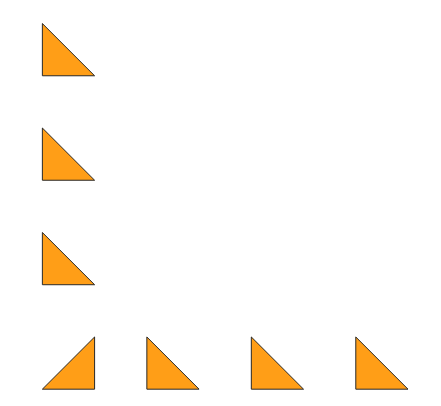
\includegraphics[width=6cm]{figures/Tugas2/1174079/no10.PNG}
		\centering
		\caption{Hasil No 10, NPM saya adalah 1174079, maka hasil modulus 8 dari NPM 1174079 adalah 7, jadi membuat bidang segitaga siku-siku dan angka kedua terakhir di NPM saya dalah 7 maka saya akan membuat 7 buah segitiga siku siku}
	\end{figure}
\end{enumerate}
\subsection{Link}
	https://youtu.be/sQsoc58IR2Y